% !TeX program = lualatex
% !TeX root = main.tex
\renewcommand*{\dictumwidth}{0.5\textwidth}
\setchapterpreamble[u]{%
	\dictum[Bill Gates%\footnotemark
]{``One thing I find myself wondering about is whether we shouldn't try and make the `ACPI' extensions somehow Windows specific. [\dots]

Or maybe we could patent something related to this.''}}
\chapter{Interfaces}
\label{chap:interfaces}
\bigskip
\textit{In this chapter, there will be a basic introduction to the different used interfaces in order to trace the processor states, beginning with ACPI, following cpufreq and cpuidle.}
%\footnotetext{\url{http://antitrust.slated.org/www.iowaconsumercase.org/011607/3000/PX03020.pdf}}

\bigskip
\lettrine[lines=2, lhang=.1, lraise=.1]{M}{odern} computer systems have plenty of ways to interact with the hardware. Of course they need to, in order to provide a fully functional and working system. The main communication between the OS and the hardware (or their firmware) is hidden for the normal computer user. But application programmer can access hardware, either direct or with one of the many generic kernel subsystems hiding hardware details and providing the main hardware functions.

%
%
\section{Advanced Configuration and Power Interface}
\label{sec:acpi}
The Advanced Configuration and Power Interface (ACPI) is a specification describing hard- and software interfaces for the implementation of OS based power management (OSPM), where the OS controls the ``power saving features'' of the devices. This is necessary considering that only the OS has all the information to efficiently send devices to sleep without harming the performance. ACPI is the successor of APM (Advanced Power Management), where only the devices themselves could control their energy saving features.

ACPI even defines its own source and machine languages: the ``ACPI Source Language'' (ASL) and the ``ACPI Machine Language'' (AML).

ACPI defines different levels of operation (operating states), composed of a letter and a number. The letter defines the region of operation and the number is an indication of the saved energy; the higher the number the more power will be saved, but latency returning to a ``lower number'' increases\cite{acpi}.\\[2em]

\noindent
Here is a short overview of the system states and what they mean:

\begin{description}
\item[G-states] Global system state definitions
	\begin{description}
	\item[G0] Working
	\item[G1\,=\,S-states] Sleeping\\
The computer appears off, but power consumption is not zero. OS context is saved and work can be resumed without rebooting.

The common sleep-states are known under suspend-to-disk (``hibernation'') and suspend-to-memory (``standby''), where the OS context is saved to disk or RAM.
	\item[G2\,=\,S5] Soft Off\,/\,Standby\\
Power consumption is minimal. No OS context is saved---system must be restarted to return to working state.
	\item[G3] Mechanical Off\\
Power consumption is zero by means of a mechanical switch. The system can be disassembled safely.
	\item[Legacy] is only used while booting or when the OS is not capable of ACPI. The device then uses its own power policy, similar to APM.
	\end{description}
\item[D-states] Device power state definitions\\device states can be applied to nearly any device on any bus. They range from D0 (Fully-On) to D3 (Off). The meaning of the states in-between is defined by each device class, and may not be defined at all. They can be thought of S-states for devices.
\item[P-states] Device and processor performance state definitions\\
	Today, P-states in processors are generally the specification of DVFS. Table \ref{tbl:pstates} shows examples for P-states.
	\begin{description}
	\item[P0] Delivers the most performance, but consumes also the most power.
	\item[Pn] Processors and devices can define up to 16 P-states, all with the same idea of limiting performance in order to save power.
	\end{description}
\item[C-states] Processor power state definitions\\
	Practically the S-states for the processor
	\begin{description}
	\item[C0] Processor is executing instructions---it is not sleeping.
	\item[Cn] different processors may implement different C-states. They can also differ in the implementation of the same state. All together is the general characteristic that a higher number implies lower power consumption but a longer wakeup-time. Not all processors report all their C-states to the OS.
	\end{description}
\end{description}
%
\newpage
\noindent
Figure \ref{fig:acpi} shows an overview of these states and how they interact which each other.

%
\begin{figure}[h]
	\centering
%	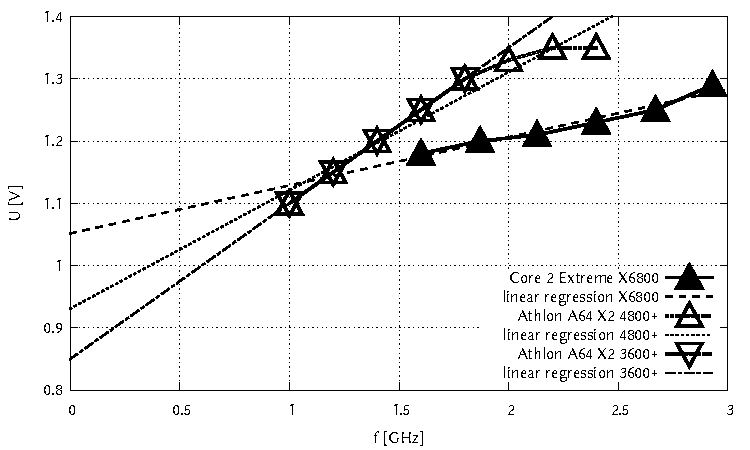
\includegraphics[width=\linewidth]{pix/pstates/pstates}
	% !TeX program = lualatex
% !TeX root = ../../main.tex
\begin{tikzpicture}[shorten >=1pt, thick, out=10, in=170, relative]
\draw 	(0,0) node[circle, minimum size=5em, inner sep=5pt, draw] (L) {Legacy}
		(5em,5em) node[circle split, minimum size=5em, inner sep=5pt, draw] (G3) 
			{G3 \nodepart{lower} \small{Mech Off}}
		(5em,-5em) node[circle split, minimum size=5em, inner sep=5pt, draw] (G2) 
			{G2 (S5) \nodepart{lower} \small{Soft Off}}
		(10em,0) node[circle split, minimum size=5em, inner sep=5pt, draw] (G0) 
			{G0 (S0) \nodepart{lower} \small{Working}}
		(13em,5em) node (Power) 
			{\small{Power Off}}
		(20em,0) node[circle split, minimum size=5em, inner sep=5pt, draw] (G1)
			{G1 \nodepart{lower} \small{Sleeping}}


		(0,-10em) node[circle split, minimum size=5em, inner sep=5pt, draw] (C0)
			{C0 (Px) \nodepart{lower} \small{CPU}}
		(10em,-10em) node[circle, minimum size=5em, inner sep=5pt] (C1)
			{\ldots}
		(20em,-10em) node[circle split, minimum size=5em, inner sep=5pt, draw] (Cn)
			{Cn \nodepart{lower} \small{CPU}}
;
\begin{scope}[circle, node distance=0em and 0em]
		\node[above right=of G1, draw] (S1) {S1};
		\node[right=of G1, draw] (S2) {S2};
		\node[below right=of G1, draw] (S3) {S3};
		\node[below=of G1, draw] (S4) {S4};

%		\node[above left=of C0, draw] (P0) {P0};
%		\node[left=of C0, draw] {\vdots};
%		\node[below left=of C0, draw] {Pn};
\end{scope}

		\draw[->] (G1) to node[below, sloped] {\small{Wake Event}} (G0);
		\draw[->] (L) to (G0);
		\draw[->] (G0) to (L);
		\draw[->] (G2) to (L);
		\draw[<-] (L) to (G3);
		\draw[->] (G3) to (G0);
		\draw[->] (G0) to (G2);
		\draw[->] (G2) to (G0);
		\draw[->] (G0) to (G1);
		\draw[<-] (G3) to (Power);

		\draw[->] (C0) to (C1);
		\draw[->, out=15, in=165, relative] (C0) to (Cn);
		\draw[->] (C1) to (Cn);
		\draw[->] (C1) to (C0);
		\draw[->, out=15, in=165, relative] (Cn) to (C0);
		\draw[->] (Cn) to (C1);
\end{tikzpicture}
\newcommand*\Captiontext{ACPI state transition overview}
	\caption[\Captiontext]{\Captiontext\cite{acpi}}
	\label{fig:acpi}
\end{figure}
%

%
\begin{table}[h]
	\caption[P-state examples]{P-state examples\cite{techarp}}
	\label{tbl:pstates}
	\centering
	\begin{tabular}{lccc}
\hiderowcolors
		\toprule
			&Core 2 Extreme X6800&Athlon A64 X2 4800+&Athlon A64 X2 3600+\\
			&[GHz / V]&[GHz / V]&[GHz / V]\\
		\midrule
\showrowcolors
			P0&2.93 / 1.2875&2.4 / 1.350&1.8 / 1.30\\
			P1&2.67 / 1.2500&2.2 / 1.350&1.6 / 1.25\\
			P2&2.40 / 1.2250&2.0 / 1.325&1.4 / 1.20\\
			P3&2.13 / 1.2125&1.8 / 1.300&1.2 / 1.15\\
			P4&1.87 / 1.2000&1.6 / 1.250&1.0 / 1.10\\
			P5&1.60 / 1.1750&1.4 / 1.200&--\\
			P6&--&1.2 / 1.150&--\\
			P7&--&1.0 / 1.100&--\\
		\bottomrule
	\end{tabular}
\end{table}
%

%
%
\section{CPUFreq}
CPUFreq is the generic kernel subsystem for managing processor P-states and was merged in kernel 2.6.9. It aims to provide a clean interface, where architecture-specific details (driver) are isolated from the generic power management policies (governor).\cite{cpufreq, ondemand}

%
\subsection{Driver}
Drivers are the interface to the processor. They must implement specific functions, like listing the available target frequencies or the frequency-change-mechanism. Providing information about the processor, e.\,g. the transition latencies or the minimum\,/\,maximum frequencies, is a duty of the driver, too. These informations are either hard-coded and general, or retrieved through the MSR of the processor. ``Machine Specific Registers'' or ``Model Specific Registers'' are a direct interface to the CPU for configuration and getting information. They can only be accessed with root-privileges and are, as the name suggests, processor dependent. MSR can be used with the assembly instructions \lstinline!RDMSR! (reads MSR) or \lstinline!WRMSR! (writes MSR).

As driver are very processor dependent, they also have to check weather they can work with the given CPU or not.

%
\subsection{Governor}
Governor are fully driver-independent and the power management policies that decide when\,/\,if to change the processor frequency.

The following governor are merged into the kernel and deliver quite a variety of policies to chose from.

\subsubsection{Performance}
The ``performance''-governor sets the CPU statically to the highest frequency within the borders of \lstinline!scaling_min_freq! and \lstinline!scaling_max_freq!.

\subsubsection{Powersave}
The ``powersave''-governor sets the CPU statically to the lowest frequency within the borders of \lstinline!scaling_min_freq! and \lstinline!scaling_max_freq!.

\superpar
The ``performance''- and ``powersave''-governors are not changing the frequency. They can be useful in some situations---hot summers or phases where latency is crucial---but they essentially disable DVFS by locking the frequency.

\subsubsection{Userspace}
The ``userspace''-governor allows the user, or any userspace program running with UID \lstinline!root!, to set the CPU to a specific frequency by making a sysfs file \lstinline!scaling_setspeed! available.

\subsubsection{Ondemand}
The ``ondemand''-governor aggressively sets the CPU depending on the current usage. It mainly switches to the highest frequency in order to complete the task and then switches instantly to the lowest. This tactic is also called ``race-to-idle''. To do this the CPU must have the capability to switch the frequency very quickly.

\subsubsection{Conservative}
The ``conservative''-governor, much like the ``ondemand''-governor, sets the CPU depending on the current usage.  It differs in behaviour in that it gracefully increases and decreases the CPU speed rather than jumping to the maximum speed the moment there is any load on the CPU. This behaviour is more suitable in a battery powered environment. 

\superpar
The ``ondemand''- and ``conservative''-governors have some preferences controlling their behaviour. These so called tuneables can be found in the CPUFreq-sysfs interface found in the appendix\,\ref{sec:cpufreqsysfs}.

%
\subsection{Programming interface}
CPUFreq also offers a C\,/\,C++ programming interface by including \lstinline!<cpufreq.h>! and linking against the \lstinline!libcpufreq!-library.

The following listing shows an abstract from the interface-specification used later in the implementation.
%
\begin{lstlisting}[%
	language=C,%
	caption={libcpufreq abstract},%
	%label={lst:freq},%
	numbers=left,%
	firstnumber=68]
/* determine current CPU frequency
 * - _kernel variant means kernel's opinion of CPU frequency
 * - _hardware variant means actual hardware CPU frequency,
 *    which is only available to root.
 */

extern unsigned long cpufreq_get_freq_kernel(unsigned int cpu);
extern unsigned long cpufreq_get_freq_hardware(unsigned int cpu);
\end{lstlisting}


% *
% * returns 0 on failure, else frequency in kHz.

%
%
\section{CPUIdle}
Like CPUFreq ``controls'' the P-states, CPUIdle is the generic kernel subsystem managing the C-states reported by ACPI---some BIOS hide deeper C-states. The maximum number of C-states the Linux kernel can handle can be found under \lstinline!/proc/acpi/processor/*/power!, for example \lstinline!max_cstate:C8!. This value represents not the number of C-states implemented in the used hardware\cite{powertop}. CPUIdle was merged in kernel 2.6.24. Exactly like CPUFreq it separates architecture-specific details (driver) from the architecture-independent implementation (governor).\cite{cpuidle, cpuidlepaper, lwn:cpuidle, cpuidle:intel}

The following governor are merged into the kernel.

\subsubsection{ladder}
The ``ladder''-governor works fine with periodic tick-based kernels. It checks every tick if it can go in a deeper idle state or not. This step-wise model works not very well with tickless kernels, because without a periodic timer tick it may not get a chance to use a deeper idle state whenever it goes idle.

\subsubsection{menu}
The ``menu''-governor on the other hand can handle this. It looks at different parameters like what the expected sleep time is (as provided by the tickless kernel), latency requirements, previous C-state residency and \lstinline!max_cstate! requirement and then picks the deepest possible idle state straight away.

%
\subsection{sysfs}
Global information can be found under\\[1em]
%
\noindent
\lstinline!$ ls -l /sys/devices/system/cpu/cpuidle!
\begin{multicols}{2}
\begin{itemize}
\renewcommand{\labelitemi}{\drsh}
\item \lstinline!current_driver!\\
	name of the current driver
\item \lstinline!current_governor_ro!\\
	name of the current governor
\end{itemize}
\end{multicols}
%

\noindent
Specific information per CPU X can be found under\\[1em]
%
\noindent
\lstinline!$ ls -l /sys/devices/system/cpu/cpuX/cpuidle!
%
\begin{multicols}{2}
\begin{itemize}
\renewcommand{\labelitemi}{\drsh}
\item \lstinline!state0!
\item \lstinline!state1!
\item \lstinline!state2!
\item \lstinline!state3!
\end{itemize}
\end{multicols}
%

\newpage
\noindent
\lstinline!$ ls -l /sys/devices/system/cpu/cpuX/cpuidle/state0!
%
%\todo{looks a bit empty, and the following description is hard to read due to the descriptive names}
%
%There are some descriptive files, like \lstinline!desc! and \lstinline!name! containing name of and description about the idle state. The exit latency is kept in \lstinline!latency!, while the consumed power, the total time spent in this state and the number of times this state was entered are in \lstinline!power!, \lstinline!time! and \lstinline!usage!.
%
\begin{multicols}{2}
\begin{itemize}
\renewcommand{\labelitemi}{\drsh}
\item \lstinline!desc!\\
	idle state description
\item \lstinline!latency!\\
	latency time exiting this state, in microseconds
\item \lstinline!name!\\
	idle state name
\item \lstinline!power!\\
	power consumed in this state
\item \lstinline!time!\\
	time spent in this state, in microseconds
\item \lstinline!usage!\\
	number of times this state was entered
\end{itemize}
\end{multicols}
%

\superpar
Figure~\ref{fig:cpufreqidle} gives a simple overview over the CPUFreq- and CPUIdle-framework, pointing out the general similarity. Up to now, these two frameworks are working absolutely independent from each other\cite{scheduler}.
%
\begin{figure}[ht]
	\centering
	%\hfill %
		\subfloat[CPUIdle]{% !TeX program = lualatex
% !TeX root = ../../main.tex
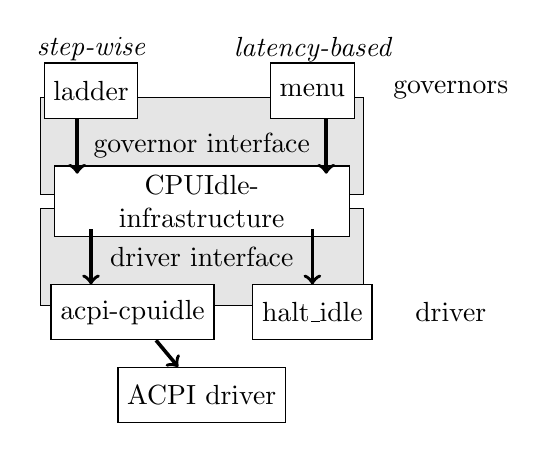
\begin{tikzpicture}[every node/.style={text centered}]
		\draw (0em, -2em)		node[draw, fill=gray!20%]
, text width=11em, minimum height=3.5em]
				{driver interface}

			(0em, 2em)		node[draw, fill=gray!20%]
, text width=11em, minimum height=3.5em]
				{governor interface}

			(0em, 0em)		node[draw, fill=white%]
, text width=10em, minimum height=2em] (cpuidle)
				{CPUIdle-infrastructure}



			(-4em, 4em)		node[draw, fill=white%]
, minimum height=2em] (ladder)
				{ladder}			
			(-4em, 5.5em)	node[font=\itshape] {step-wise}


			(4em, 4em)		node[draw, fill=white%]
, minimum height=2em] (menu)
				{menu}			
			(4em, 5.5em)	node[font=\itshape] {latency-based}




			(9em, 4em)	node {governors}
			(9em, -4em)	node {driver}
			
			(-2.5em, -4em)	node[draw%]
, minimum height=2em, fill=white] (acpiidle)
				{acpi-cpuidle}




			(0em, -7em)	node[draw%]
, minimum height=2em, fill=white] (acpidriver)
				{ACPI driver}

			(4em, -4em)	node[draw%]
, minimum height=2em, fill=white] (haltidle)
				{halt\_idle}
;

	\draw[->, line width=1.3pt] (4.5em, 3em) -- (4.5em, 1em);%(menu) -- (cpuidle);
	\draw[->, line width=1.3pt] (-4.5em, 3em) -- (-4.5em, 1em);%(ladder) -- (cpuidle);

	\draw[<-, line width=1.3pt] (4em, -3em) -- (4em, -1em);%(haltidle) -- (cpuidle);
	\draw[<-, line width=1.3pt] (-4em, -3em) -- (-4em, -1em);%(acpiidle) -- (cpuidle);
	\draw[<-, line width=1.3pt] (acpidriver) -- (acpiidle);
\end{tikzpicture}}
	\hfill % alternativ auch \hspace{1cm} für genaue Angaben
		\subfloat[CPUFreq]{% !TeX program = lualatex
% !TeX root = ../../main.tex
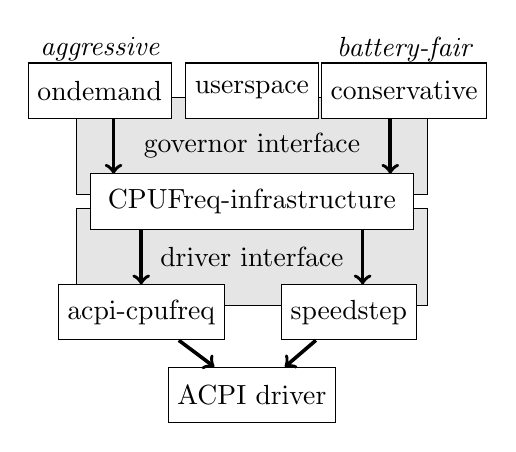
\begin{tikzpicture}[every node/.style={text centered}]
		\draw (0em, -2em)		node[draw, fill=gray!20%]
, text width=12em, minimum height=3.5em]
				{driver interface}

			(0em, 2em)		node[draw, fill=gray!20%]
, text width=12em, minimum height=3.5em]
				{governor interface}

			(0em, 0em)		node[draw, fill=white%]
, text width=11em, minimum height=2em] (cpuidle)
				{CPUFreq-infrastructure}



			(-5.5em, 4em)		node[draw, fill=white%]
, minimum height=2em] (ondemand)
				{ondemand}			
			(-5.5em, 5.5em)	node[font=\itshape] {aggressive}


			(5.5em, 4em)		node[draw, fill=white%]
, minimum height=2em] (conservative)
				{conservative}			
			(5.5em, 5.5em)	node[font=\itshape] {battery-fair}

			(0em, 4em)		node[draw, fill=white%]
, minimum height=2em] (userspace)
				{userspace}	



%			(-11em, 4em)	node {governors}
%			(-11em, -4em)	node {driver}
			
			(-4em, -4em)	node[draw%]
, minimum height=2em, fill=white] (acpifreq)
				{acpi-cpufreq}

(3.5em, -4em)	node[draw%]
, minimum height=2em, fill=white] (speedstep)
				{speedstep}



			(0em, -7em)	node[draw%]
, minimum height=2em, fill=white] (acpidriver)
				{ACPI driver}
			
;

	\draw[->, line width=1.3pt] (5em, 3em) -- (5em, 1em);%(menu) -- (cpuidle);
	\draw[->, line width=1.3pt] (-5em, 3em) -- (-5em, 1em);%(ladder) -- (cpuidle);

	\draw[<-, line width=1.3pt] (4em, -3em) -- (4em, -1em);%(haltidle) -- (cpuidle);
	\draw[<-, line width=1.3pt] (-4em, -3em) -- (-4em, -1em);%(acpiidle) -- (cpuidle);
	\draw[<-, line width=1.3pt] (acpidriver) -- (acpifreq);
	\draw[<-, line width=1.3pt] (acpidriver) -- (speedstep);
\end{tikzpicture}}
	%\hfill %
	\caption[Design Overview CPUIdle\,/\,CPUFreq]{Design Overview CPUIdle\,/\,CPUFreq\cite{overview}}
	\label{fig:cpufreqidle}
\end{figure}
%

%
%
\section{Intelligent Platform Management Interface}
IPMI enables system administrators to manage computer systems and monitor their operation through a set of standardized computer system interfaces.

It is possible to communicate with a distant computer over a serial connection or a local network with IPMI. Error messages can be sent with SNMP (simple network management protocol). Direct BIOS access over LAN is also possible.

The interfaces are working independently from any OS and allow system administration without installed OS or even in standby-mode. More possibilities arise while the computer system is running, for example starting\,/\,stopping the computer, or disabling the on-\,/\,off- or reset-button.

The core of IPMI is the so called baseboard management controller (BMC). Other Controller for monitoring special hardware can be connected to it over the IPMB (intelligent platform management bus). This way monitoring fan speeds or the voltages of CPUs can be done mainly by hardware with low performance impact on the OS or other running software.
The BMC is already integrated on recent server mainboards\cite{ipmi}.

%Open source management software for IPMI exists:
%IPMItool (BSD-Lizenz)
%GNU FreeIPMI (GPL)


\superpar
While IPMI focuses on remote maintenance and large data centers with special hardware, lm-sensors\footnote{\url{http://www.lm-sensors.org/}} concentrates on providing off-the-shelf hardware monitoring support for Linux. Lm-sensors is widely used in private servers and small test clusters made up of standard PC components.

The minimum update interval of lm-sensors is only 1.5 seconds, whereas IPMI is event-based and can deliver sensor data within 50\,milliseconds. For that reason, and because most recent clusters are using IPMI, integration of lm-sensors has low priority.